\documentclass{ceurart}
\sloppy
\usepackage{listings}
\lstset{breaklines=true}

\graphicspath{{svgs/}}

\def\species#1{\textit{#1}}
\def\term#1{`#1'}
\def\property#1{\textit{#1}}
\def\curie#1{\textsf{#1}}
\def\function#1{\textit{#1}}

\begin{document}
\copyrightyear{2024}
\copyrightclause{Copyright for this paper by its authors.
  Use permitted under Creative Commons License Attribution 4.0
  International (CC BY 4.0).}

\conference{Proceedings of the International Conference on Biomedical
Ontologies 2024, July 17--19, 2024, Enschede, The Netherlands}

\title{(Re-)bridging the anatomy ontologies with SSSOM}

\author[1]{Damien Goutte-Gattat}[%
orcid=0000-0002-6095-8718,
email=dpg44@cam.ac.uk,
]
\cormark[1]
%\fnmark[1]
\address[1]{University of Cambridge, Downing Street, Cambridge, CB2 3DY, United Kingdom}

\author[2]{Nicolas Matentzoglu}[
orcid=0000-0002-7356-1779,
email=nicolas.matentzoglu@gmail.com,
]
\address[2]{Semanticly, Athens 10563, Greece}

\cortext[1]{Corresponding author.}
%\fntext[1]{These authors contributed equally.}

\begin{abstract}
Ontologies that describe the anatomical structures and cell types of model
organisms are critically required for the annotation and successful
exploitation of high-throughput datasets. The Uberon ontology (for anatomical
structures) and the Cell Ontology (CL, for cell types) jointly aim to provide a
consistent ontology that can be used across a wide range of species, by
leveraging existing species-centric anatomy ontologies to construct a single
integrated multi-species ontology. In this paper, we describe how we overhauled
the integration mechanism between Uberon, CL, and the species-centric
ontologies by using the newly devised SSSOM (``Simple Standard for Sharing
Ontological Mappings'') standard to manage the mappings between all concerned
ontologies.
\end{abstract}

\begin{keywords}
  Anatomy ontologies \sep
  mappings \sep
  cross-species studies
\end{keywords}

\maketitle

\section{Introduction}

One of the prerequisites for the reuse and reanalysis of datasets from
high-throughput experimental methods --~such as single-cell RNA
sequencing datasets~-- beyond their lab of origin is the annotation of
samples and results with standardised terms. That is, we need controlled
vocabularies to properly record information such as the exact techniques
used, the organs or tissues from which the experimental samples were
taken, or the cell types that were identified. Several ontologies have
been developed for this kind of purpose, such as the Experimental Factor
Ontology (EFO) to annotate experimental methods~\cite{malone2010}, the
Drosophila Anatomy Ontology (FBbt) to annotate anatomical structures and
cell types in \species{D.~melanogaster}~\cite{costa2013}, the Worm
Anatomy Ontology (WBbt) to do the same in
\species{C.~elegans}~\cite{lee2003}, etc. Most of those ontologies are
grouped under the umbrella of the OBO Foundry~\cite{jackson2021}.

However, comparing datasets across species additionally requires that
the ontology terms used to annotate the datasets are themselves
comparable. For example, comparing a dataset of mouse blood cells with a
dataset of fly hemocytes requires that some link (relationship) exist
between the term representing the concept of blood in mice and the term
representing the concept of hemolymph in flies. Ideally, this would in
turn require that a single cross-species ontology be used for all
datasets, containing all the terms needed to represent all anatomical
structures and cell types with their species-specific variations,
organised in a consistent hierarchy.

\section{The Uberon strategy for a multi-species ontology}

Building a single cross-species anatomy ontology from the ground up,
with terms suitable for all the model organisms, would be a gigantic
task, requiring lots of species-specific expertise that would be hard to
gather in a single project.  Instead, a more practical approach was
adopted by the Uberon project~\cite{mungall2012a} which, rather than
attempting to describe the anatomy of every model organism, leverages
the existing species-specific anatomy ontologies. Uberon aims to provide
a ``core'' anatomy ontology that describes anatomical structures in a
species-neutral way, along with ``bridges'' that allow to integrate the
more precise terms from the species-specific ontologies
(Figure~\ref{fig:bridges}). The result of merging the Uberon core
ontology with the species-specific ontologies along with the
corresponding bridges is a product called \emph{composite-metazoan}
(hereafter CM), a single, consistent cross-species ontology. The Cell
Ontology (CL), an ontology of cell types, follows the same
approach~\cite{diehl2016}, and is automatically included in Uberon's CM
product.

\begin{figure}
  \centering
  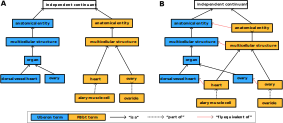
\includegraphics[width=\linewidth]{bridges}
  \caption{Uberon and the Drosophila Anatomy Ontology (FBbt) maintain
  their own hierarchy of terms separately. Simply merging the two
  ontologies together \textbf{(A)} would result in a hierarchy that is
  apparently unified but is, in effect, split in two independent
  branches that are solely connected by BFO's \term{independent
  continuant} root term, preventing any meaningful use. \textbf{(B)}
  Bridging axioms (dotted red arrows) between Uberon and FBbt allow to
  connect \species{Drosophila}-specific terms to their taxon-neutral
  counterparts, thereby crossing the gap between the two branches.}
  \label{fig:bridges}
\end{figure}

To implement this strategy, Uberon maintains a set of cross-ontology
mappings, which are used to determine where the terms from the
species-specific ontologies should be placed in the overall Uberon
hierarchy. Across ontologies of the OBO Foundry, the typical method to
represent and maintain mappings is to use cross-references (or,
informally, ``xrefs''). It’s a very simple method where, to map a term
$T_A$ in an ontology A to a term $T_B$ in a foreign ontology B, $T_A$ is
annotated with a \property{oboInOwl:hasDbXref} property, whose value is
the short identifier (``CURIE'') of $T_B$. As part of the Uberon release
pipeline, a Perl script automatically extracts those cross-references
and generates the bridge files needed to integrate the species-specific
ontologies.

While simple, the cross-reference method has several limitations. (i) It
does not allow to record any metadata about the mapping, such as: who
asserted that the two terms should be mapped? On what basis? When was
the mapping reviewed?  (ii) The method does not allow for any nuance:
either two terms are mapped or they are not, without room to express
more subtle relations. (iii) Cross-references are embedded within the
ontology itself, and are therefore not easily reusable by third parties.
(iv) Cross-references have no clear and universally agreed upon meaning.
When two terms are mapped to each other, the meaning of the mapping is
left unspecified, and typically has to be inferred from the ontologies
that are being mapped (for example, a mapping between the
species-neutral Uberon and the \species{Drosophila}-specific FBbt can be
inferred to be a cross-species mapping). This is made worse by the fact
that cross-references in OBO ontologies are used for many different
things beyond just mappings; for example, when used to annotate a term
definition, cross-references typically attribute a source for the
definition, akin to a citation in an academic paper.

\section{New approach to cross-ontology mappings}

We have devised a new approach to maintain and use cross-ontology
mappings in Uberon, centred around three axes: (i) the use of a new
format to represent the mappings, (ii) the creation of dedicated mapping
relations, and (iii) the development of new tools to manipulate the
mappings and, in particular, derive OWL axioms from them.

\subsection{The SSSOM standard}

The Simple Standard for Sharing Ontological Mappings (SSSOM) is a
recently devised standard specifically intended to facilitate the
exchange of semantic mappings~\cite{matentzoglu2022b}. It allows
mappings to be treated as first-class data entities and to attach to
them a range of metadata such as provenance and licensing information.
The standard defines a common data model to represent mappings as well
as two distinct serialisation formats to store and transport instances
of the model: a JSON-based format and a TSV-based format. The TSV format
has been specifically designed to be easily manipulatable both by
standard spreadsheet software (for editing by curators) and by common
science libraries and tools (for use by data scientists and engineers).
At least two independent implementations of the standard are available:
SSSOM-Py and SSSOM-Java, for the Python and Java programming languages,
respectively. In addition, several ontology-related tools have started
to add direct support for the format, such as the Ontology Access
Kit~\cite{mungall2023} and the Ontology Development
Kit~\cite{matentzoglu2022a}. The community resource Biomappings also
provides its mappings in SSSOM, among other formats~\cite{hoyt2023}.

\subsection{New mapping relations for cross-species mappings}

One of the benefits brought by the SSSOM standard is the possibility to
use highly specific mapping predicates to express precisely the intended
meaning of a mapping. While many mapping sets don’t actually need this,
and can use common mapping predicates such as those from the SKOS
vocabulary~\cite{bechhofer2009} (\property{skos:exactMatch},
\property{skos:narrowMatch}, etc.), cross-species mappings are an
example of an application where the common predicates are not
sufficient. For example, let us consider a mapping between the FBbt term
for neuron (\curie{FBbt:00005106}, representing a neuron in a fruit fly)
and the corresponding term in the Cell Ontology (\curie{CL:0000540},
representing a neuron in any species): clearly it would not be correct
to state that a fly neuron is the same concept as a neuron in any other
species --~the two terms are not interchangeable, so
\property{skos:exactMatch} is not a suitable mapping predicate.  A
slightly more correct predicate could be \property{skos:narrowMatch},
because is it true that a fly neuron is a narrower concept than a
species-neutral neuron; but a sensory neuron (\curie{CL:0000101}) is
also a narrower concept than a generic neuron, yet the relation between
\term{sensory neuron} and \term{neuron} is of a different nature than
the relation between \term{fly neuron} and \term{(species-neutral)
neuron}.

Overall we believe that cross-species mappings are \emph{sui generis}
mappings and that they warrant the use of dedicated mapping predicates
to reflect that fact. We therefore expanded the SEMAPV vocabulary,
specifically established for use with SSSOM~\cite{matentzoglu2022}, with
four new mapping predicates (Figure~\ref{fig:relations}) that mirror
existing SKOS predicates but are specifically intended for cases where
the subject and object of a mapping belong to different taxonomic
groupings.

\begin{figure}
  \centering
  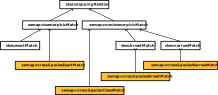
\includegraphics[width=.8\linewidth]{relations}
  \caption{Excerpt of the semantic mapping vocabulary (SEMAPV), with the
  new mapping relations (yellow) introduced to specifically represent
  cross-species mappings.}
  \label{fig:relations}
\end{figure}

\subsection{Deriving OWL bridges from SSSOM}

Even as SSSOM adoption spreads rapidly, it is likely that many tools
will remain unable to directly exploit SSSOM sets in the foreseeable
future.  Therefore, when mappings are stored in the SSSOM format, we
need to be able to convert them into OWL axioms that can be used by any
ontology manipulation tool. To that effect, we have developed a SSSOM
plugin for ROBOT, the standard tool used to manipulate OBO
ontologies~\cite{jackson2019}.  The plugin is built on top of the Java
implementation of the SSSOM standard and provides a \emph{sssom:inject}
command that takes a SSSOM mapping set as input, derives OWL axioms from
the mappings, and injects them into an ontology.

Rather than hardcoding the logic for deriving the axioms --~which would
have been efficient but would have made the logic harder to modify and
re-use~-- we designed a small domain-specific language (DSL), named
SSSOM/T-OWL (``SSSOM/Transform-to-OWL''), that allows users to describe
which mappings in a set should be transformed into OWL axioms and what
kind of axioms should be produced.

The SSSOM/T-OWL language is organised around the single concept of
``transformation rules''. A rule is made of two elements
(Table~\ref{tab:sssomt}): a filter (or selector) to decide whether the
rule should apply to a given mapping; and either a preprocessor, to
modify a mapping on the fly, or a generator, to produce a OWL axiom from
the mapping.

\begin{table}
  \caption{SSSOM/T-OWL filters, preprocessors, and generators}
  \label{tab:sssomt}
  \begin{tabular}{ll}
    \toprule
    SSSOM/T-OWL element & Examples\\
    \midrule
    Atomic filter & \verb|predicate==skos:exactMatch|\\
    Negated filter & \verb|!subject==UBERON:*|\\
    Intersection filter & \verb|subject==UBERON:* && predicate==skos:exactMatch|\\
    Union filter & \verb+subject==UBERON:* || subject==CL:*+\\
    \midrule
    Inversion preprocessor & \verb|-> invert()|\\
    Exclusion preprocessor & \verb|-> stop()|\\
    Assignation preprocessor & \verb|-> assign("subject_source", "uberon.owl")|\\
    Replacement preprocessor & \verb|-> replace("mapping_tool", "pattern", "replacement")|\\
    \midrule
    Generic axiom generator & \verb|-> create_axiom("%subject_id EquivalentTo: %object_id")|\\
    Subject annotation generator & \verb|-> annotate_subject(oboInOwl:hasDbXref, "%object_curie")|\\
    Object annotation generator & \verb|-> annotate_object(oboInOwl:hasDbXref, "%subject_curie")|\\
    \bottomrule
  \end{tabular}
\end{table}

Filters allow the value of any of the SSSOM metadata slots to be
compared with a target value and to discard any mapping with a different
value. A basic form of wildcard matching is supported, where a filter
can select mappings with a value that starts with the same prefix as the
target value. Individual filters can be combined to select mappings
based on more than just one metadata slot; they can also be negated, so
that a filter that would select a given set of mappings would, after
negation, instead select the complementary set of mappings.

Preprocessors allow a mapping to be modified before it is used by
subsequent rules. Possible modifications include inverting a mapping
(the subject becomes the object and vice-versa) and changing some of the
mapping's metadata. A preprocessor can also be used to completely remove
a mapping from the set, so that no further rule will be applied to this
mapping.

Finally, the generators take the selected mapping and turn it into an
axiom.  The most important generator function is
\function{create\_axiom}, which can produce an arbitrary axiom described
by an expression in Manchester syntax~\cite{patel-schneider2012}. Other
generators allow classes of the ontology to be annotated with any of the
available mappings metadata.

Of note, the current implementation of the SSSOM/T-OWL language cleanly
separates the OWL generators from the filters and the preprocessing
functions.  This makes it easy to create other domain-specific languages
similar to SSSOM/T-OWL, using the same overall syntax, the same filters
and the same preprocessors, but that generate objects other than OWL
axioms.

\section{Application of the approach to the Uberon pipeline}

With the components described in the previous section in place, we
overhauled the pipeline that builds Uberon's \emph{composite-metazoan}
product (Figure~\ref{fig:pipeline}).

\begin{figure}
  \centering
  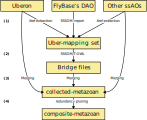
\includegraphics[width=.4\linewidth]{pipeline}
  \caption{Uberon's new pipeline. A Single SSSOM set, encompassing
  mappings with all target species, is created by extracting
  old-style cross-references from both Uberon and several other
  species-specific anatomy ontologies --~except FlyBase's FBbt, which
  already provides a ready-to-use SSSOM set (1). The resulting set is
  processed by the Uberon SSSOM/T-OWL ruleset (2) to create the bridge
  files, which are then merged along with the source ontologies to
  create the \emph{collected-metazoan} ontology (3). The final
  \emph{composite-metazoan} is created (4) by pruning redundant terms
  using a custom ROBOT plugin.}
  \label{fig:pipeline}
\end{figure}

\subsection{Collecting the mappings}

Rather than migrating all of Uberon mappings to SSSOM at once, we have
adopted a phased approach, in which we have used the mappings between
Uberon and FBbt as a test bed in a preliminary phase. Uberon/FBbt
mappings were initially maintained as cross-references within Uberon, as
for all the other Uberon mappings. We migrated them to a SSSOM mapping
set that we now maintain on the FBbt side: existing FBbt
cross-references in Uberon were extracted from the ontology and
converted into SSSOM mappings using the newly minted
\property{semapv:crossSpeciesExactMatch} predicate (all existing
cross-references were for exact mappings, since that was the only kind
of mapping allowed by the cross-reference system), that are now
published alongside the FBbt ontology itself.

Mappings between Uberon and the other species-specific anatomy
ontologies beyond FBbt are still currently maintained as
cross-references either within Uberon or within the species-specific
ontologies. They are extracted and converted to SSSOM dynamically as
part of Uberon's release pipeline. In a second phase, which we have not
started yet, we will migrate those mappings fully to SSSOM, as was done
for the FBbt mappings.

\subsection{Applying the transformation rules}

Regardless of their origin, all mappings between Uberon, CL, and the
species-specific ontologies are processed by a single large SSSOM/T-OWL
ruleset that contains all the required logic to generate the bridging
axioms. A typical rule in this ruleset is the following:

\begin{lstlisting}
(subject==UBERON:* || subject==CL:*) && object==FBbt:*
  && predicate==semapv:crossSpeciesExactMatch
  -> create_axiom('%object_id EquivalentTo: %subject_id and
                   (BFO:0000050 some NCBITaxon:7227)');
\end{lstlisting}

That rule can be literally understood as: a mapping between a Uberon (or
CL) term and a FBbt term and that uses the
\property{semapv:crossSpeciesExactMatch} predicate must be transformed
into an equivalence axiom that states that the FBbt term is equivalent
to the intersection of the Uberon (or CL) term and an existential
restriction over \curie{BFO:0000050} (\term{part of}) and
\curie{NCBITaxon:7227} (\term{Drosophila melanogaster}).

All axioms produced by the SSSOM/T-OWL ruleset are saved into a separate
bridge file for each foreign ontology.

\subsection{Building the composite-metazoan ontology}

Once the bridge files have been generated, an intermediate ontology
(\emph{collected-metazoan}) is built by merging together Uberon itself,
the Cell Ontology, all the species-specific ontologies, and their
corresponding bridges. Finally, \emph{composite-metazoan} itself is
derived from this intermediate product by applying some custom logic
(implemented in a small, dedicated ROBOT plugin) to ``prune'' redundant
terms and replace them with equivalent anonymous class expressions.

The details of this last operation are beyond the scope of this paper,
but as an example, let us consider the FBbt term \term{ovary}
(\curie{FBbt:00004865}): it is mapped to the Uberon term \term{ovary}
(\curie{UBERON:0000992}), so \emph{collected-metazoan} contains the
following axiom:

\begin{lstlisting}
FBbt:00004865 EquivalentTo: UBERON:0000992 and
                            (BFO:0000050 some NCBITaxon:7227)
\end{lstlisting}

The ``pruning'' operation leading to \emph{composite-metazoan} consists
of replacing all occurrences of \curie{FBbt:00004865} by the anonymous
expression it is equivalent to. So the following axiom, which states
that the \term{oviduct} (\curie{FBbt:00004911}) is \term{continuous
with} (\curie{RO:0002150}) the fly ovary:

\begin{lstlisting}
FBbt:00004911 SubClassOf: RO:0002150 some FBbt:000004865
\end{lstlisting}

gets rewritten as:

\begin{lstlisting}
FBbt:00004911 SubClassOf: RO:0002150 some (UBERON:0000992 and
                          (BFO:0000050 some NCBITaxon:7227))
\end{lstlisting}

\section{Conclusion}

In this project, we have (i) expanded the SEMAPV vocabulary so that
cross-species mappings can be specifically represented in SSSOM; (ii)
introduced a domain-specific language (SSSOM/T-OWL) to allow converting
SSSOM mappings into arbitrary OWL axioms; (iii) implemented said
language in a new ROBOT plugin to inject SSSOM-derived axioms into a OWL
ontology; (iv) used those new tools to update the integration mechanism
between Uberon, CL, and the species-centric ontologies, with an approach
centered on the use of SSSOM, rather than cross-references, to manage
the mappings between the ontologies.

As a result, cross-species mappings across anatomy ontologies are now
available as a \emph{bona fide} release artefact of Uberon, provided as
a distinct file in a known location in a standard format, thereby
greatly facilitating the reuse of said mappings by any interested third
party. The logic for deriving the bridge files (needed to correctly
merge Uberon and the species-specific ontologies), now expressed in the
SSSOM/T-OWL language, is itself consequently more easily maintainable
and reusable.

While several aspects of this project (most notably the precise
SSSOM/T-OWL rules we use) are specific to the needs of Uberon, we
believe the general approach of maintaining mappings as SSSOM sets and
transforming them into OWL bridges using a simple DSL could be
generalised to any project that requires integrating several ontologies
together.

\begin{acknowledgments}
This work was supported by grant BB/T014008 from the UK Biotechnology
and Biological Sciences Research Council (BBSRC) and the US National
Science Foundation Directorate of Biological Sciences (NSF/BIO).
\end{acknowledgments}

\bibliography{sssomt}

\appendix

\section{Online Resources}

The SSSOM-Java project, which implements both the SSSOM standard and the
SSSOM/T-OWL language described in this paper, is hosted on
\href{https://github.com/gouttegd/sssom-java/}{GitHub}.

Uberon artefacts concerned by this project are available under the
following permanent URLs:

\begin{tabular}{ll}
\hline
Artefact & PURL\\
\hline
SSSOM mapping set & \url{http://purl.obolibrary.org/obo/uberon/uberon.sssom.tsv}\\
Bridge to ontology \emph{X} & \url{http://purl.obolibrary.org/obo/uberon/bridge/uberon-bridge-to-X.owl}\\
Composite Metazoan & \url{http://purl.obolibrary.org/obo/uberon/composite-metazoan.owl}\\
\hline
\end{tabular}

\end{document}
